\documentclass[tikz,border=8pt]{standalone}
\usepackage{pgfplots}
\pgfplotsset{compat=1.18}
\usetikzlibrary{arrows.meta}
\begin{document}
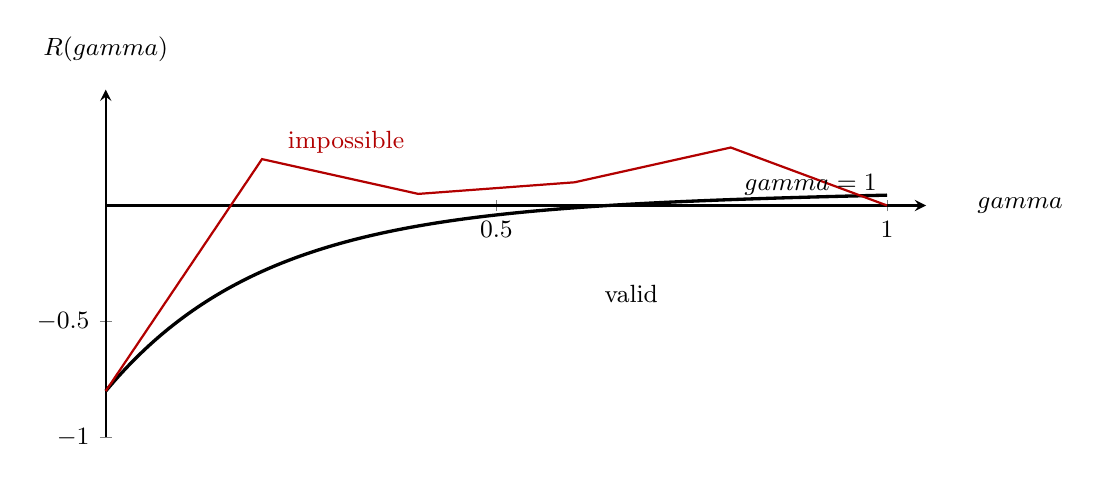
\begin{tikzpicture}[font=\small]
\begin{axis}[
    width=12cm,
    height=6cm,
    xmin=0,xmax=1.05,
    ymin=-1,ymax=0.5,
    axis lines=middle,
    xlabel={$\\gamma$},
    ylabel={$R(\\gamma)$},
    xtick={0,0.5,1},
    ytick={-1,-0.5,0},
    domain=0:1,
    samples=200,
    thick,
    clip=false,
    every axis x label/.style={at={(ticklabel* cs:1.05)},anchor=west},
    every axis y label/.style={at={(ticklabel* cs:1.05)},anchor=south},
]
% valid curve (black)
\addplot[black,very thick] { -0.8*exp(-5*x)+0.05*x };
% impossible curve (red)
\addplot[red!70!black,thick] coordinates {(0,-0.8) (0.2,0.2) (0.4,0.05) (0.6,0.1) (0.8,0.25) (1,0)};
\node[red!70!black,anchor=south west] at (axis cs:0.22,0.18) {impossible};
\node[black,anchor=north east] at (axis cs:0.72,-0.3) {valid};
\node[anchor=south east] at (axis cs:1,0) {$\\gamma=1$};
\end{axis}
\end{tikzpicture}
\end{document}
